\subsection{Definition Smart Home Zentrale}
 	\begin{figure}[ht!]
 		\centering
 		\begin{minipage}[t]{0.3\linewidth}
 			\centering
 			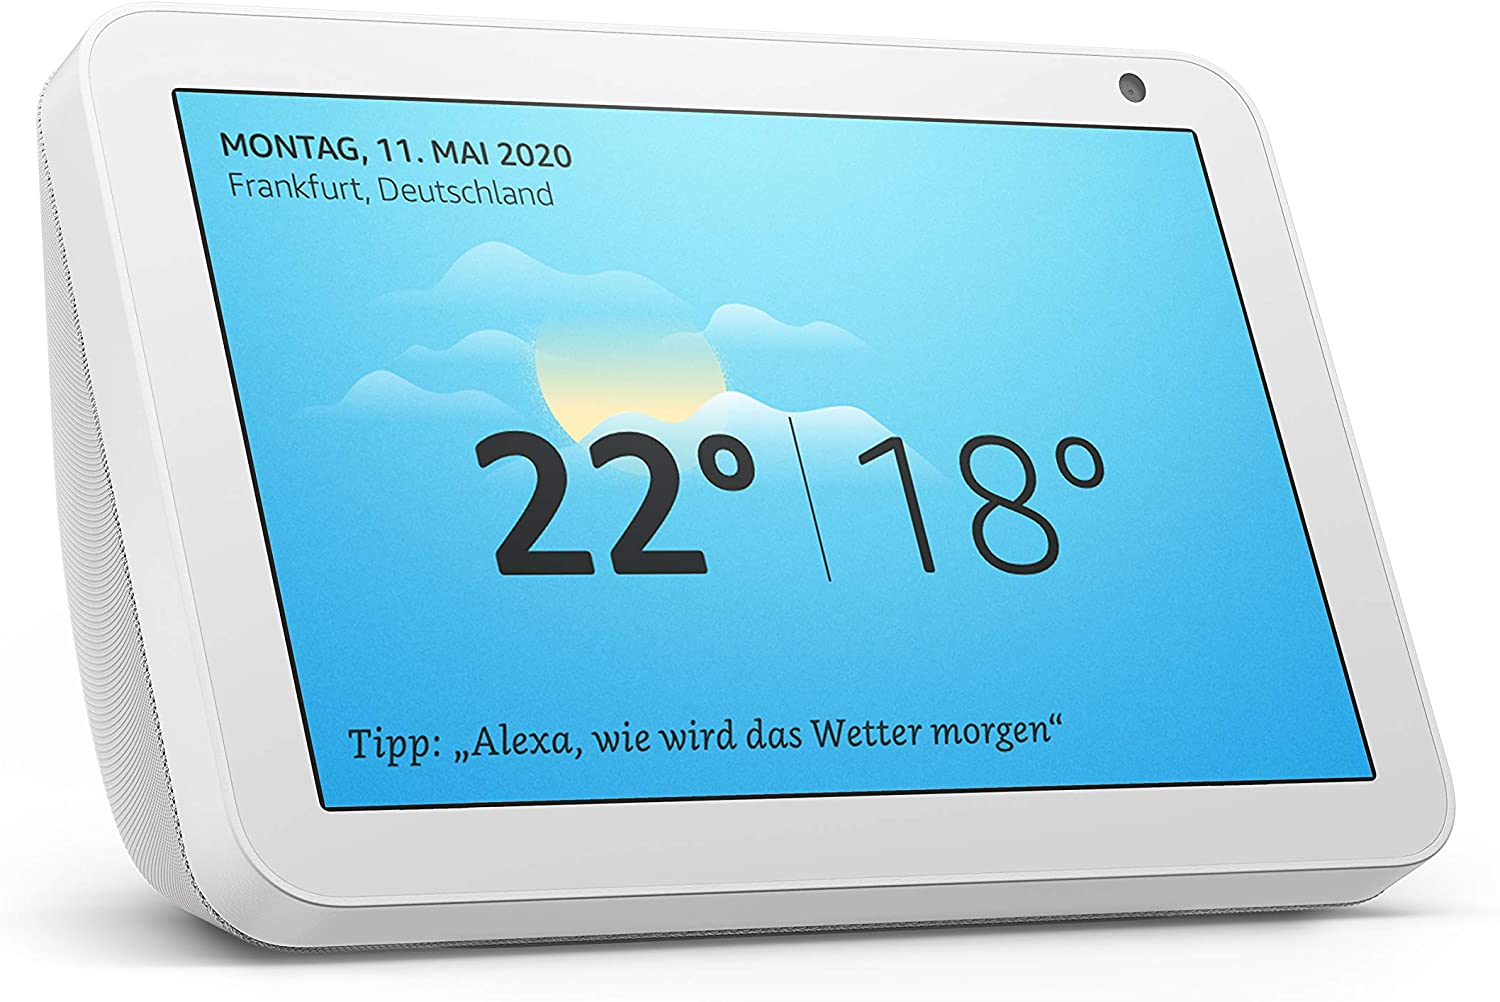
\includegraphics[width=0.7\textwidth]{img/alexa_echo_show8.jpg}
 			\caption[Amazon Alexa Echo Show 8]{Amazon Alexa Echo Show 8}
 			\label{fig:alexa-echo-show8}
 		\end{minipage}
 		\hfill
 		\begin{minipage}[t]{0.3\linewidth}
 			\centering
 			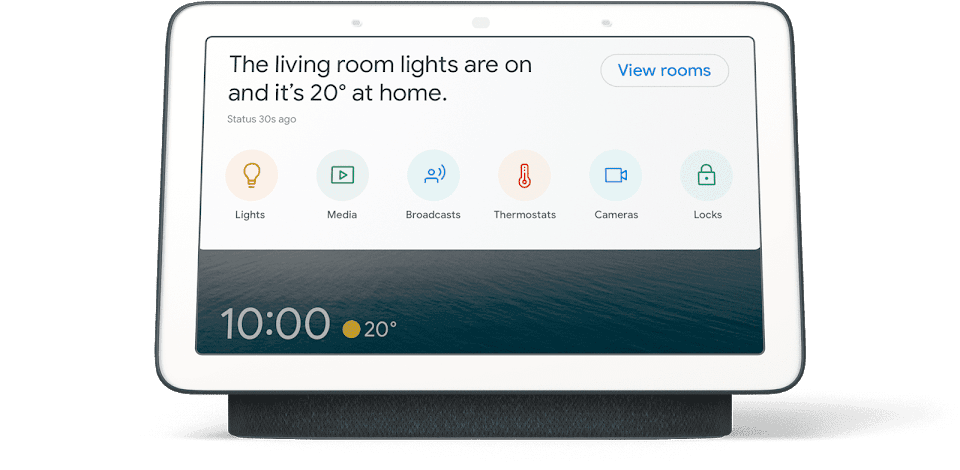
\includegraphics[width=0.7\textwidth]{img/google_nest_hub.png}
 			\caption[Google Nest Hub]{Google Nest Hub}
 			\label{fig:google-nest-hub}
 		\end{minipage}
 		\hfill
 		\begin{minipage}[t]{0.3\linewidth}
 			\centering
 			\includegraphics[width=0.7\textwidth]{img/glancr_smart_mirror.jpeg}
 			\caption[Glancr Smart Mirror]{Glancr Smart Mirror}
 			\label{fig:glancr-smart-mirror}
 		\end{minipage}
 	\end{figure}
 	\textbf{Smart Home Zentralen}, auch \textbf{Smart Hubs} oder \textbf{Smart Mirrors} genannt, sind Geräte, die als zentraler Knotenpunkt in einem Smart Home Netzwerk sitzen und dort Informationen verarbeiten, weiterleiten und darstellen können.\par
 	Diese Geräte werden von den meisten Herstellern mit und ohne Bildschirm geliefert, um entweder ein neues Smart Home aufzubauen oder ein bestehendes Smart Home zu erweitern. 
 	\begin{quote}
 	\color{quotetext}
 		Bei einem Smart-Home-Hub handelt es sich um eine schlaue Zentrale, durch die all deine intelligenten Geräte miteinander vernetzt werden – und dadurch erst wirklich ihren gesamten Leistungsumfang ausschöpfen.\footnote{Li (2017): Was ist ein Smart-Home-Hub? Alles über die intelligente Zentrale}
 	\end{quote}
Als Smart Home Zentrale können auch Software-Lösungen gezählt werden, die mit den im Netz befindlichen Smart Hubs kommunizieren und die Informationen mit Hilfe eines Web-Interfaces oder einer Smartphone-Anbindung darstellen und steuern können. Beispiele hierfür sind homeassistant.io, openHAB und Google Home.\par
	% Sollte eigentlich die 3 Logos darstellen wie die Geräte darüber. Macht er aber nit... 	
% 	\begin{figure}[hb]
%		\centering
% 		\begin{minipage}[t]{0.3\linewidth}
% 			\centering
% 			
\includegraphics[width=0.7\textwidth]{img/home-assistant-io_logo.png}
%			\caption[Home Assistant Logo]{Home Assistant}
%			\label{fig:hassio}
% 		\end{minipage}
% 		\hfill
% 		\begin{minipage}[t]{0.3\linewidth}
%			\centering
% 			
\includegraphics[width=0.7\textwidth]{img/openhab_logo.png}
% 			\caption[openHAB Logo]{openHAB}
%			\label{fig:openhab}
% 		\end{minipage}
% 		\hfill
%		\begin{minipage}[t]{0.3\linewidth}
%			\centering
%			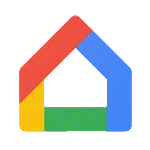
\includegraphics[width=0.7\textwidth]{img/google-cast_logo.png}
% 			\caption[Google Home Logo]{Google Home}
% 			\label{fig:googlehome}
% 		\end{minipage}
% 	\end{figure}
 	\newpage
	% Hier den Rest eintragen...
	% Folgend erst mal der allgemeine Aufbau nach dem einen Beispiel, das ich in Telegram geteilt hab...